\def\i{\item}
\graphicspath{{../pictures/c5/}}
%\chapter{MỘT SỐ YẾU TỐ THỐNG KÊ VÀ XÁC SUẤT}
\newpage
\section{BÀI TẬP CUỐI CHƯƠNG V}
\subsection{SƠ ĐỒ TƯ DUY TỔNG KẾT CHƯƠNG V}
\begin{center}
	\includegraphics[width=1\linewidth]{doc1.pdf}
\end{center}
\subsection{CÂU HỎI TRẮC NGHIỆM}
\begin{ex}
	Kết quả điểm tổng kết cuối học kì I của một học sinh được ghi lại như sau
	\vskip 0.1cm
	\resizebox{\columnwidth}{!}{\begin{tabular}{|p{0.055\linewidth}|p{0.055\linewidth}|p{0.055\linewidth}|p{0.055\linewidth}|p{0.055\linewidth}|p{0.055\linewidth}|p{0.055\linewidth}|p{0.055\linewidth}|p{0.055\linewidth}|p{0.055\linewidth}|p{0.055\linewidth}|p{0.065\linewidth}|}
	\hline
	Toán&	Ngữ văn&	Ngoại ngữ 1&	GD CD&	CN&	Tin học&	KH TN&	LS \& ĐL&	Giáo dục thể chất&	Nghệ thuật&	HĐ TN HN&	ND GD của địa phương\\
	\hline
	8,6&	8,3&	7,5&	8,6&	8,5&	8,4&	8,6&	8,7&	Đ&	Đ&	Đ&	Đ\\
	\hline
	\end{tabular}}
	\vskip 0.1cm
	Các môn học không được đánh giá bằng số liệu là
	\choice
	{Giáo dục thể chất, Nghệ thuật, HĐTNHN}
	{Toán, Ngữ văn, Ngoại ngữ 1, GDCD, CN, Tin học, KHTN, LS\&ĐL}
	{Giáo dục thể chất, Nghệ thuật, ND GD của địa phương}
	{Giáo dục thể chất, Nghệ thuật, HĐTNHN, ND GD của địa phương}
\end{ex}
\begin{ex}
	Điểm kiểm tra môn Toán của một nhóm học sinh được ghi lại theo bảng sau
	\begin{center}
		\begin{tabular}{|c|c|c|c|c|}
			\hline
			Điểm&	5&	6&	8&	9\\
			\hline
			Số học sinh&	2&	4&	3&	2\\
			\hline
		\end{tabular}
	\end{center}
	Nhóm này có bao nhiêu học sinh?
	\choice{28}{11}{10}{76}
\end{ex}
\begin{ex}
	Cho dãy dữ liệu sau:
	
	Tên một số truyện cổ tích Việt Nam: Sọ Dừa, Thạch Sanh, Cây tre trăm đốt, Thầy bói xem voi.  
	
	Dữ liệu không hợp lý trong dãy dữ liệu trên là:
	\choice
	{Sọ Dừa}
	{Thạch Sanh}
	{Thầy bói xem voi}
	{Cây tre trăm đốt}
\end{ex}
\begin{ex}
	Cho dãy dữ liệu sau:
	
	Diện tích ($km^2$) của 4 tỉnh/thành phố: Hà Nội, Vĩnh Phúc, Bắc Ninh, Quảng Ninh lần lượt là  3358,6; 1235,2; 822,7; 6,1782.
	
	Dữ liệu không hợp lý trong dãy dữ liệu trên là:
	\choice{3358,6}{1235,2}{822,7}{6,1782}
\end{ex}
\begin{ex}
	Kết quả kiểm tra môn Toán của học sinh lớp   được cho trong bảng sau:
	\begin{center}
		\begin{tabular}{|l|c|c|c|c|c|c|c|c|c|c|c|}
			\hline
			Điểm & 1&2&3&4&5&6&7&8&9&10\\
			\hline
			Số HS &0&3&2&1&7&8&9&7&4&1\\
			\hline
		\end{tabular}
	\end{center}
	Số học sinh đạt điểm 7 là
	\choice{5}{9}{8}{13}
\end{ex}
\begin{ex}
	Cho biểu đồ thể hiện kết quả học lực học kì I của học sinh khối 6 trường THCS X
	\begin{figure}[H]
		\centering
		\vspace*{-5pt}
		\captionsetup{labelformat= empty, justification=centering}
		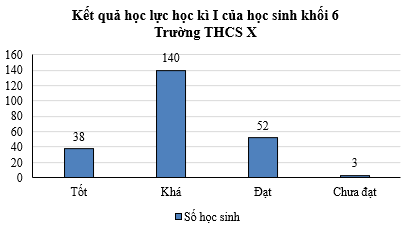
\includegraphics[width=0.5\linewidth]{18}
		\vspace*{-10pt}
	\end{figure}
	Tổng số học sinh khối 6 của trường THCS X là: 
	\choice{38}{140}{52}{243}
\end{ex}
\begin{ex}
	Câu 7. Cho biểu đồ dưới đây:
	\begin{figure}[H]
		\centering
		\vspace*{-5pt}
		\captionsetup{labelformat= empty, justification=centering}
		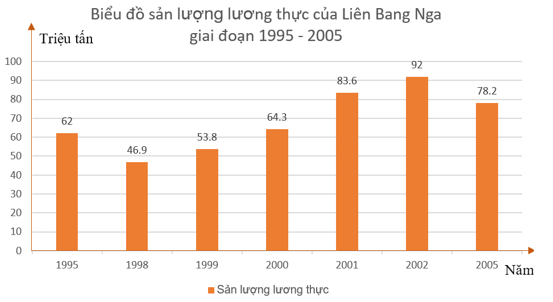
\includegraphics[width=0.5\linewidth]{19}
		\vspace*{-10pt}
	\end{figure}
	Trong giai đoạn $1995-2005$ ở Liên Bang Nga, năm nào có sản lượng lương thực thấp nhất?
	\choice{1995}{1998}{2000}{2005}
\end{ex}
\begin{ex}
	Biểu đồ tranh sau đây biểu diễn số lượng dâu tây thu hoạch của 3 tổ học sinh lớp $6B$ trong đợt đi dã ngoại
	\begin{center}
		\begin{tabular}{|l|l|}
			\hline
			Tổ 1 & \\
			\hline
			Tổ 2 & \\
			\hline
			Tổ 3 & \\
			\hline
		\end{tabular}
	
	\vspace*{5pt}
	(Mỗi ứng với 2kg dâu tây)
	\end{center}
	Bảng thống kê được lập từ biểu đồ tranh trên là: 
	\choice
	{\begin{tabular}{|c|c|c|c|}
			\hline
			Tổ & 1&2&3\\
			\hline
			Số lượng dâu tây(kg) & 4&2&3\\
			\hline
	\end{tabular}}
	{\begin{tabular}{|c|c|c|c|}
			\hline
			Tổ & 1&2&3\\
			\hline
			Số lượng dâu tây(kg) & 8&4&6\\
			\hline
	\end{tabular}}
	{\begin{tabular}{|c|c|c|c|}
			\hline
			Tổ & 1&2&3\\
			\hline
			Số lượng dâu tây(kg) & 6&4&6\\
			\hline
	\end{tabular}}
	{\begin{tabular}{|c|c|c|c|}
			\hline
			Tổ & 1&2&3\\
			\hline
			Số lượng dâu tây(kg) & 8&6&6\\
			\hline
	\end{tabular}} 
\end{ex}
\begin{ex}
	Từ biểu đồ cột kép thể hiện số huy chương vàng và tổng số huy chương đạt được của các quốc gia tham dự SEA games 31 (\textit{Theo NGUỒN : SEAGAMES31 ngày 23/5/2022})
	\begin{figure}[H]
		\centering
		\vspace*{-5pt}
		\captionsetup{labelformat= empty, justification=centering}
		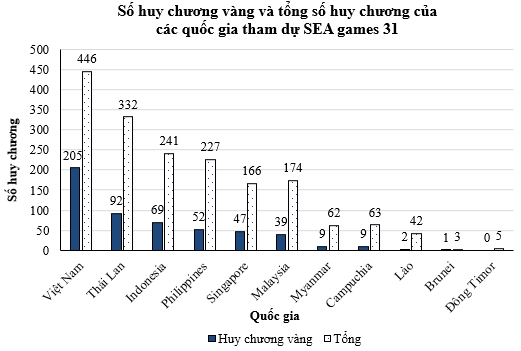
\includegraphics[width=0.5\linewidth]{20}
		\vspace*{-10pt}
	\end{figure}
	Đoàn thể thao của quốc gia nào đã có số huy chương vàng trên tổng số huy chương quốc gia đó đạt được là nhiều nhất
	\choice{Việt Nam}{Thái Lan}{Indonesia}{Campuchia}
\end{ex}
\begin{ex}
	Từ biểu đồ cột kép về điểm kiểm tra các môn của Mai và Bình
	\begin{figure}[H]
		\centering
		\vspace*{-5pt}
		\captionsetup{labelformat= empty, justification=centering}
		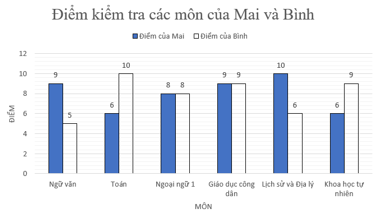
\includegraphics[width=0.5\linewidth]{21}
		\vspace*{-10pt}
	\end{figure}
	Ta có bảng thống kê là:
	\choice
	{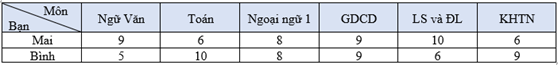
\includegraphics[width=0.9\linewidth]{b1}}
	{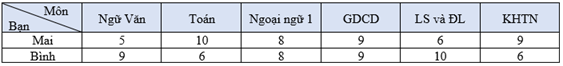
\includegraphics[width=0.9\linewidth]{b2}}
	{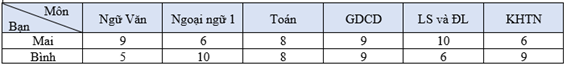
\includegraphics[width=0.9\linewidth]{b3}}
	{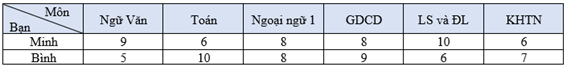
\includegraphics[width=0.9\linewidth]{b4}}
\end{ex}
\begin{ex}
	Dưới đây là bảng thống kê kết quả bình chọn các hoạt động trong buổi dã ngoại của học sinh lớp $6A$:
	\begin{center}
		\begin{tabular}{|c|c|c|c|c|}
			\hline
			Hoạt động&	Cắm trại&	Đạp xe&	Đạp vịt&	Ca hát\\
			\hline
			Số học sinh&  	19&	9&	14&	8\\
			\hline
		\end{tabular}
	\end{center}
	Trong các biểu đồ sau, biểu đồ nào biểu diễn đúng nội dung bảng thống kê trên?
	\choice
	{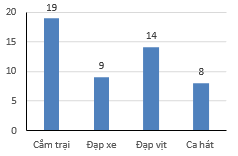
\includegraphics[width=0.3\linewidth]{22a}}
	{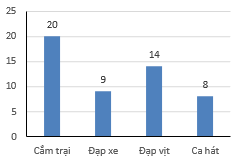
\includegraphics[width=0.3\linewidth]{22b}}
	{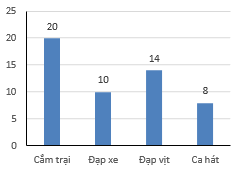
\includegraphics[width=0.3\linewidth]{22c}}
	{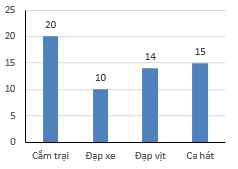
\includegraphics[width=0.3\linewidth]{22d}}
\end{ex}
\begin{ex}
	Một cuộc điều tra về vệ sinh khu phố cho thấy có 60 người sử dụng xà phòng rửa tay, 40 người chỉ rửa tay bằng nước sạch, còn lại là số người không rửa tay trước khi ăn. Biết số người không rửa  tay trước khi ăn chiếm  $\dfrac{1}{6}$ tổng số người được điều tra.
	
	Cho mỗi   ứng với 10 người. Khi đó số biểu tượng   cần điền vào trong biểu đồ tranh dưới đây là bao nhiêu?
	\begin{center}
		\begin{tabular}{|l|l|}
			\hline
			Sử dụng xà phòng rửa tay& \\
			\hline	      
			Chỉ rửa tay bằng nước sạch& \\
			\hline	    
			Không rửa tay trước khi ăn	&?\\
			\hline
		\end{tabular}
	\end{center}
	\choice{20}{6}{2}{10}
\end{ex}
\begin{ex}
	Nếu tung một đồng xu  30 lần liên tiếp, có 16  lần xuất hiện mặt N thì xác suất thực nghiệm xuất hiện mặt S bằng bao nhiêu?
	\choice{$\dfrac{7}{15}$}{$\dfrac{3}{8}$}{
	$\dfrac{5}{8}$}{$\dfrac{8}{15}$}
\end{ex}
\begin{ex}
	Quân và Việt cùng thực hiện trò chơi tung đồng xu  2000 đồng (nếu tung được mặt sấp thì kí hiệu S, nếu tung được mặt ngửa thì kí hiệu N) và ghi lại kết quả như sau:
	\begin{center}
		\begin{tabular}{|l|c|c|c|c|c|c|c|c|c|c|}
			\hline
			Lần &1&2&3&4&5&6&7&8&9&10\\
			\hline
			Quân&S&S&N&S&N&N&N&S&N&S\\
			\hline
			Việt&N&N&S&S&S&N&S&N&N&S\\
			\hline
		\end{tabular}
	\end{center}
	Xác suất thực nghiệm của sự kiện cả hai bạn cùng tung được mặt sấp là
	\choice{$\dfrac{3}{10}$}{
	$\dfrac{1}{10}$}{$\dfrac{1}{5}$}{$\dfrac{2}{5}$}
\end{ex}
\begin{ex}
	Bạn Lâm gieo một con xúc xắc 100 lần và ghi lại số lần xuất hiện của mặt ghi số chấm như sau:
	\begin{center}
		\begin{tabular}{|l|c|c|c|c|c|c|}
			\hline
			Mặt ghi số chấm& 	1&	2&	3&	4&	5&	6\\
			\hline
			Số lần xuất hiện&	16&	18&	18&	17&	15&	16\\
			\hline
		\end{tabular}
	\end{center}
	Xác suất thực nghiệm xuất hiện mặt có số chấm là số chẵn là:
	\choice{$\dfrac{18}{100}$}{$\dfrac{17}{100}$}{$\dfrac{16}{100}$}{$\dfrac{51}{100}$}
\end{ex}
\subsection{BÀI TẬP TỰ LUẬN}
\Opensolutionfile{loigiaichung}[loigiaichuong42]
\begin{bt}
	Trong hội thi “Người Làm Vườn Tài Năng” cấp huyện, Bác Hùng (đội trưởng) được ban tổ chức yêu cầu thống kê số tuổi của các thành viên trong đội mình. Bác Hùng đã liệt kê số tuổi của các thành viên trong đội của mình như sau:
	\begin{center}
		\begin{tabular}{|c c c c c c c c c|}
			\hline
			50 & 73& 30& 45& 70& 18& 21& 50& 43 \\
			50& 30& 45& 70& 18& 65& 50& 65& 50\\
			50&45&40&20&30&44&73&51&49\\
			\hline
		\end{tabular}
	\end{center}
	\begin{enumerate}[a),leftmargin=*]
		\i Hãy nêu đối tượng thống kê và tiêu chí thống kê?
		\i Bác Hùng thông báo số người ở độ tuổi trên 45 tuổi bằng 3 lần số người có độ tuổi từ 45 tuổi trở xuống. Vậy thông báo này là đúng hay sai? Vì sao?
	\end{enumerate}
	\begin{loigiaichuong42}
		\begin{enumerate}[a),leftmargin=*]
			\i Đối tượng thống kê ở đây là:
			\begin{enumerate}[+,leftmargin=*]
				\i Các thành viên trong đội của Bác Hùng
				\i Tiêu chí thống kê là số tuổi của mỗi người trong đội.
			\end{enumerate}
			\i Có 9 người từ  45 tuổi trở xuống
			
			Và có 18 người từ 45 tuổi trở lên.
			
			Vậy thông báo của bác Hùng là sai 
		\end{enumerate}
	\end{loigiaichuong42}
\end{bt}
\begin{bt}
	Tổ trưởng Minh đưa bảng theo dõi điểm kiểm tra giữa kỳ( theo thang điểm  ) của các thành viên trong tổ cho các bạn như sau:
	\begin{center}
		\begin{tabular}{|c c c c c c c c|}
			\hline
			10 & 3&9&9&8&8&9&10\\
			10&7&8&7&5&7&6&7\\
			\hline
		\end{tabular}
	\end{center}
	\begin{enumerate}[a),leftmargin=*]
		\i Trong tổ của Minh có bao nhiêu thành viên.\\
		Nêu đối tượng thống kê và tiêu chí thống kê.
		\i Trong tổ Minh, có bao nhiêu bạn đạt điểm trên TB\\
		Có bao nhiêu bạn đạt điểm khá--giỏi (từ  7 điểm trở lên)
		\i Nếu Minh được 8  điểm thì trong tổ điểm của Minh có phải cao nhất không?
	\end{enumerate}
	\begin{loigiaichuong42}
		\begin{enumerate}[a),leftmargin=*]
			\i Tổ của Minh có 16  học sinh.
			\begin{enumerate}[--,leftmargin=*]
				\i Đối tượng thống kê ở đây là: Các thành viên trong tổ của Minh.
				\i Tiêu chí thống kê là số điểm kiểm tra giữa kì môn Toán của các thành viên trong tổ.
			\end{enumerate}
			\i Lập bảng thống kê:
			\begin{center}
				\begin{tabular}{|l|c|c|c|c|c|c|c|}
					\hline
					Số điểm & 10 & 9&8&7&6&5&3\\
					\hline
					Số người& 3&3&3&4&1&1&1\\
					\hline
				\end{tabular}
			\end{center}	 
			Từ bảng thống kê trên ta thấy:
			\begin{enumerate}[+,leftmargin=*]
				\i Tổ của Minh có 14  bạn đạt điểm trên trung bình( trên 5 điểm)
				\i Có 13 bạn đạt điểm khá giỏi
			\end{enumerate}
			Trong tổ của Minh có điểm 10 điểm là điểm cao nhất nên Minh được 8 điểm chưa phải là điểm cao nhất.
		\end{enumerate}
	\end{loigiaichuong42}
\end{bt}
\begin{bt}
	Tờ Live Science đã liệt kê 9 loại virus nguy hiểm nhất thế giới, dựa trên nguy cơ tử vong, số ca tử vong và khả năng trở thành một mối đe dọa trong tương lai của chúng đó là: Virus Marburg, Virus Ebola, Virus dại, Virus HIV, Virus đậu mùa, Virus cúm, Virus SARS, Virus MERS, Virus SARS--CoV--2 (Virus Corona). 
	
	Dưới đây là biểu đồ thể hiện tỉ lệ tử vong và năm xuất hiện của 4 trong số 9 loại virus đó
	\begin{figure}[H]
		\centering
		\vspace*{-5pt}
		\captionsetup{labelformat= empty, justification=centering}
		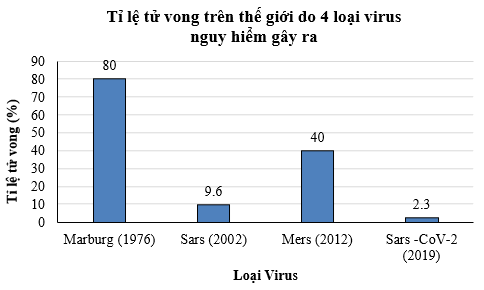
\includegraphics[width=0.5\linewidth]{23}
		\vspace*{-10pt}
	\end{figure}
	Em hãy quan sát biểu đồ và trả lời các câu hỏi sau:
	\begin{enumerate}[a),leftmargin=*]
		\i Trong 4 loại virus trên, virus nào gây ra tỉ lệ tử vong cao nhất? Virus đó xuất hiện năm nào?
		\i Thế giới phát hiện ra loại virus SARS vào năm bao nhiêu, so sánh tỉ lệ tử vong của SARS với Sars--CoV--2.
		\i Em hãy nêu một vài hiểu biết của mình về sự xuất hiện của Virus Sars--CoV--2 trên thế giới? 
	\end{enumerate}
	\begin{loigiaichuong42}
		\begin{enumerate}[a),leftmargin=*]
			\i Trong 4 loại virus trên, virus gây ra tỉ lệ tử vong cao nhất là Marburg, virus đó xuất hiện năm 1976.
			\i Thế giới phát hiện ra loại virus SARS vào năm 2002
			\begin{enumerate}[+,leftmargin=*]
				\i Tỉ lệ tử vong của SARS là  $9,6\%$ 
				\i Tỉ lệ tử vong của Sars--CoV--2 là $2,3 \%$ 
			\end{enumerate}
			Vậy tỉ lệ tử vong của SARS lớn hơn Sars--CoV--2.
			\i Chủng virus SARS--CoV--2 thuộc cùng một họ với SARS--CoV, được gọi là virus Corona, xuất hiện lần đầu vào tháng 12 năm 2019 tại thành phố Vũ Hán của Trung Quốc. COVID--19 do virus SARS--CoV--2 gây ra có tỉ lệ tử vong ước tính khoảng $2,3\%$ (tính đến tháng 3.2020). Các triệu chứng thường gặp bao gồm sốt, ho khan và khó thở và có thể tiến triển thành viêm phổi.
		\end{enumerate}
	\end{loigiaichuong42}
\end{bt}
\begin{bt}
	Dưới đây là biểu đồ số ca mắc và tử vong của dịch Covid--19 của các khu vực trên thế giới tính đến 0 giờ ngày $31-12-2020$ (\textit{Nguồn: Worldometers}) 
	\begin{figure}[H]
		\centering
		\vspace*{-5pt}
		\captionsetup{labelformat= empty, justification=centering}
		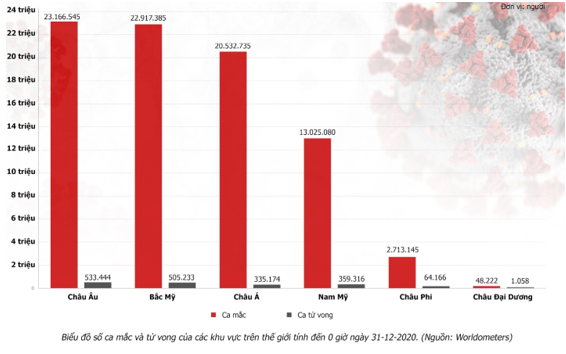
\includegraphics[width=0.5\linewidth]{24}
		\vspace*{-10pt}
	\end{figure}
	Dựa vào biểu đồ em hãy cho biết: Tính đến 0 giờ ngày $31-12-2020$
	\begin{enumerate}[a),leftmargin=*]
		\i Khu vực nào trên thế giới có số ca mắc Covid--19 cao nhất (bao nhiêu triệu người)? 
		\i Tổng số ca tử vong trên thế giới là bao nhiêu?
		\i Tính tỉ lệ tử vong so với số ca mắc của Châu Á?
	\end{enumerate}
	\begin{loigiaichuong42}
		Tính đến 0 giờ ngày $31-12-2020$
		\begin{enumerate}[a),leftmargin=*]
			\i Khu vực Châu Âu có số ca mắc Covid--19 cao nhất thế giới (23.166.545 triệu người)
			\i Tổng số ca tử vong trên thế giới là: 
			\[533444 + 505233 + 335174 + 359316 + 64166 + 1058 = 1.798.391 \text{ (triệu người)}\]  
			\i Tỉ lệ tử vong so với số ca mắc của Châu Á là:  $\dfrac{{335174}}{{20532735}} \approx 1,63\%$
		\end{enumerate}
	\end{loigiaichuong42}
\end{bt}
\begin{bt}
	TikTok là nền tảng video âm nhạc và mạng xã hội của Trung Quốc được ra mắt vào năm 2017, dành cho các thị trường bên ngoài Trung Quốc. Bởi Trương Nhất Minh, người sáng lập của ByteDance. Nó được sử dụng để tạo các video ca nhạc ngắn, hát nhép, khiêu vũ, hài kịch \ldots từ   đến   giây, và các video lặp lại ngắn từ   đến   giây được giới trẻ yêu thích. 
	
	Hình vẽ sau là biểu đồ cho biết số lượt tải TikTok trên 1 tháng tại Việt Nam từ tháng 1/2020 đến tháng 2/2021 (đơn vị là triệu lượt).
	\begin{figure}[H]
		\centering
		\vspace*{-5pt}
		\captionsetup{labelformat= empty, justification=centering}
		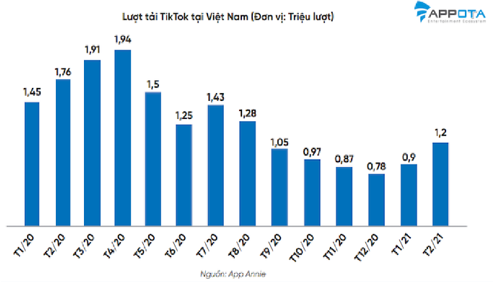
\includegraphics[width=0.5\linewidth]{25}
		\vspace*{-10pt}
	\end{figure}
	Em có được thông tin gì khi em quan sát biểu đồ này?
	\begin{loigiaichuong42}
		\begin{enumerate}[--,leftmargin=*]
			\i Đối tượng thống kê người tải TikTok tại Việt Nam trong các tháng từ tháng 1/2020 đến tháng 02/2021
			\i Tiêu chí thống kê là số lượt tải TikTok trên một tháng được thống kê từ tháng 01/2020 đến tháng 02/2021 tại Việt Nam 
			\i Vào 04/2020 số người tải TikTok cao nhất, có 1,94 triệu lượt
			\i Vào khoảng từ tháng 01/2020 đến tháng 08/2020 có số lượt tải rất cao, từ 1,25  đến 1,94 triệu lượt
			Từ tháng 09/2020 đến tháng 02/2021 số lượt tải giảm đi rõ rệt, chỉ từ 0,78 đến 1,2 triệu lượt 
			\i Tháng 12/ 2020 có số lượt tait TikTok là thấp nhất, có  lượt \ldots.
		\end{enumerate}
	\end{loigiaichuong42}
\end{bt}
\begin{bt}
	Trong hộp có 1 viên bi xanh (X), 1 viên bi đỏ (Đ) và 1 viên bi vàng (V). Hùng lấy ra lần lượt từng viên, ghi màu của viên bi rồi trả nó lại hộp. Kết quả 7 lần lấy bi cho ở bảng sau:
	\begin{center}
		\begin{tabular}{|l|c|c|c|c|c|c|c|}
			\hline
			Lần lấy thứ	&1&	2&	3&	4&	5&	6&	7\\
			\hline
			Màu viên bi&	Đ&	V&	Đ&	X&	V&	V&	X\\
			\hline
		\end{tabular}
	\end{center}
	\begin{enumerate}[a),leftmargin=*]
		\i Hãy cho biết kết quả của lần lấy bi thứ 2 và thứ 4.                                                                
		\i Hãy cho biết có bao nhiêu kết quả khác nhau có thể xảy ra trong mỗi lần lấy bi.
	\end{enumerate}        
	\begin{loigiaichuong42}
		\begin{enumerate}[a),leftmargin=*]
			\i Lần thứ 2 lấy được bi vàng, lần thứ 4 lấy được bi xanh.
			\i Có 3 kết quả khác nhau khi lấy bi là lấy được bi xanh, bi đỏ và bi vàng.
		\end{enumerate}
	\end{loigiaichuong42}
\end{bt}           
\begin{bt}
	Trong hộp có 10 tấm bìa ghi các số tự nhiên từ 1 đến 10. Lan rút ngẫu nhiên 1 tấm bìa.
	\begin{enumerate}[a),leftmargin=*]
		\i Sự kiện nào có khả năng xảy ra cao hơn trong hai sự kiện sau:
		\begin{enumerate}[+,leftmargin=*]
			\i Sự kiện A: Tấm bỉa ghi số chẵn
			\i Sự kiện B: Tấm bìa ghi số nguyên tố.
		\end{enumerate}
		\i Lan rút tấm bìa 20 lần, mỗi lần Lan ghi lại kết quả rồi lại bỏ vào hộp. Tính xác suất thực nghiệm của 2 sự kiện trên biết 9 lần xảy ra sự kiện A và 8 lần xảy ra sự kiện B. 
	\end{enumerate}
	\begin{loigiaichuong42}
		\begin{enumerate}[a),leftmargin=*]
			\i Sự kiện A có khả năng xảy ra cao hơn. Vì từ 1 đến 10 có năm số là số chẵn đó là: 2, 4, 6, 8, 10 và có bốn số là số nguyên tố đó là: 2, 3, 5, 7.
			\i Xác suất thực nghiệm của sự kiện A là: $\dfrac{9}{{20}} = 0,45$ 
			
			Xác suất thực nghiệm của sự kiện B là:  $\dfrac{8}{{20}} = 0,4$
		\end{enumerate}
	\end{loigiaichuong42}
\end{bt}
\begin{bt}
	Một cửa hàng làm phiếu khảo sát về mức độ hài lòng của một số khách hàng được lựa chọn ngẫu nhiên trong tháng thứ nhất. Kết quả thu được như sau:
	\begin{center}
		\begin{tabular}{|l|c|c|c|}
			\hline
			Mức độ hài lòng&	Không hài lòng&	Hài lòng&	Rất hài lòng\\
			\hline
			Số khách hàng&	5&	10&	5\\
			\hline
		\end{tabular}
	\end{center}
	\begin{enumerate}[a),leftmargin=*]
		\i Tính xác suất thực nghiệm của sự kiện khách hàng không hài lòng.
		\i Nhà hàng tiếp tục khảo sát trong tháng thứ hai.  Kết quả thu được như sau:
		\begin{center}
			\begin{tabular}{|l|c|c|c|}
				\hline
				Mức độ hài lòng&	Không hài lòng&	Hài lòng&	Rất hài lòng\\
				\hline
				Số khách hàng&	3&	12&	5\\
				\hline
			\end{tabular}\,\,\,\,\,\,\,\,\,
		\end{center}
		Tính xác suất thực nghiệm của sự kiện khách hàng không hài lòng sau hai tháng.
		
		Độ hài lòng của khách sau hai tháng tăng hay giảm?
	\end{enumerate}
	
	\begin{loigiaichuong42}
		\begin{enumerate}[a),leftmargin=*]
			\i Có 5 khách hàng không hài lòng trong số 20 khách hàng nên xác suất thực nghiệm là: $\dfrac{5}{{20}} = 0,25$
			\i Tổng số khách hàng không hài lòng sau hai tháng là: $5 + 3 = 8$ trong số 40 khách hàng nên xác suất thực nghiệm là:   $\dfrac{8}{{40}} = 0,2$
			
			Vì $0,2 < 0,25$ nên độ không hài lòng của khách giảm đi, tức độ hài lòng của khách tăng lên.
		\end{enumerate}
	\end{loigiaichuong42}
\end{bt}
%D. BẢNG ĐÁP ÁN CÂU HỎI TRẮC NGHIỆM
%1. D	2. B	3. C	4. D	5. B	6. D	7. B	8. B
%9. A	10. A	11. A	12. C	13. A	14. C	15. D	
\Closesolutionfile{loigiaichung}
